
\subsection{Surface Data Preprocessing}
\label{sec:data-preprocessing}

To obtain consistent sectional representations across the aerodynamic databases, the upper and lower airfoil surfaces were processed separately using local chord-normalized coordinates. The original CFD nodes were ordered by $\xi=x/c$, and nearly coincident chordwise locations were merged before interpolation. Both surface geometry and pressure coefficients were resampled using shape-preserving piecewise cubic Hermite interpolation (PCHIP) \cite{FritschButland1984}, which limits spurious overshoots when interpolating pressure distributions with steep local gradients.

A total of 100 chordwise nodes were allocated between the upper and lower surfaces. Under transonic conditions, the upper surface generally exhibits more pronounced suction peaks and sharper pressure gradients, including possible shock-induced pressure variations, whereas the lower-surface pressure distribution is typically smoother. To provide higher resolution in regions of stronger pressure variation, more nodes were assigned to the upper surface using prescribed importance weights of $\omega_u=1.8$ and $\omega_l=1.0$, resulting in 64 upper-surface and 36 lower-surface nodes.

For each surface, the chordwise nodes were concentrated near the leading edge, with the spacing increasing smoothly toward a uniform-spacing region downstream. The interval widths were prescribed using a fifth-order smoothstep function:
\begin{equation}
    w_{s,j}=1+(r_s-1)S\left(\min\left(\frac{j}{K_s},1\right)\right),\qquad S(t)=6t^5-15t^4+10t^3,
    \label{eq:chordwise-spacing}
\end{equation}
where $s\in\{u,l\}$, $j=0,\ldots,N_s-2$, $K_s=\max\{1,\lfloor\rho_s(N_s-2)\rfloor\}$, and $r_s$ controls the ratio of downstream to initial spacing. The chordwise node coordinates were obtained by normalizing the cumulative interval widths and mapping them to the prescribed sampling interval. The distribution parameters were $(\rho_u,r_u)=(0.28,5.0)$ and $(\rho_l,r_l)=(0.24,4.0)$ for the upper and lower surfaces, respectively. The resulting chordwise discretization is shown in Fig.~\ref{fig:chordwise-nodes}, which compares the node locations and adjacent-node spacing on the upper and lower surfaces.

\begin{figure}[!htb]
    \centering
    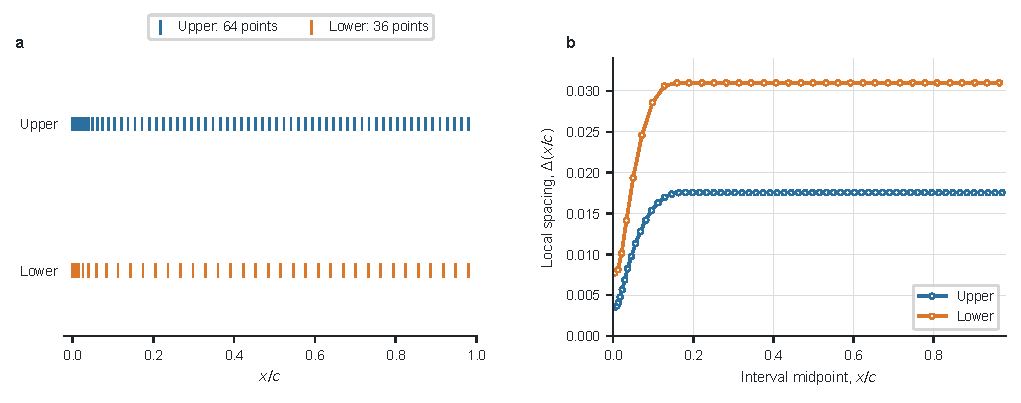
\includegraphics[width=0.94\linewidth]{II_Database_and_Preprocessing/figures/II_C_Fig07/II_C_Fig07_chordwise_nodes.pdf}
    \caption{Chordwise discretization of the upper and lower airfoil surfaces: (a) node locations and (b) adjacent-node spacing.}
    \label{fig:chordwise-nodes}
\end{figure}

For finite-wing configurations, the original CFD sectional locations were retained without additional spanwise interpolation. Following chordwise resampling, the paired infinite-span and constant-chord finite-wing pressure distributions share identical chordwise coordinates, allowing the finite-span pressure corrections in Eq.~\eqref{eq:paired-delta-cp} to be calculated by pointwise subtraction. The upper- and lower-surface pressure data were retained separately for subsequent aerodynamic modeling.
